% !TEX root = ../notes_template.tex
\chapter{Muscle Tension}\label{chp:tension}

\minitoc

The goal of this chapter is to describe how muscle fibers generate both active and passive tension. Passive tension occurs when the muscle fibers resist lengthening and can also be referred to as stretch. Active tension is what we think of when we use the term muscle contraction. The muscle fibers create active tension which generates a force that shortens (or attempts to shorten) the fiber.  The fundamental difference between passive and active tension is whether the muscle is converting chemical energy from the form adenosine triphosphate (ATP) to mechanical energy at the crossbridge site between the proteins actin and myosin. During active tension the muscle is actively converting chemical energy to mechanical energy at this crossbridge site, whereas during passive tension the muscle is not actively converting chemical energy to mechanical energy at this crossbridge site, but is still resisting a unidirectional change in length. A unidirectional change in length we mean a muscle only generates passive tension in one direction, it resists lengthening. The muscle does not generate passive tension to resist shortening. The important point here is that the difference between active tension and passive tension is not whether the muscle is shortening or lengthening. The difference is also not whether there is positive or negative $\Delta$ length. The difference is whether the muscle fiber is converting chemical energy to mechanical energy. The term we’ll use for this is activated or activation, not contracted or contraction since the term contraction tends to imply a change in length. 

\vspace{5mm}

\textbf{Objectives include:}
\begin{enumerate}
    \item Describe the structures that generate tension.
    \item Explain the role of passive tension in muscle function.
    \item Describe the sliding filament theory of active tension.
    \item Explain the role of active tension in muscle function.
    \item Explain the underlying mechanisms and implications of the length-tension and force-velocity relationships.
   \item Apply the concept of muscle tension to the analysis of patient/client problems related to the generation of muscle force.
\end{enumerate}

\section{Anatomy of Tension}

The anatomy of tension focuses on the structures that are (mostly \footnotemark{}\footnotetext{First, the focus is on the muscle fiber not the muscle \textit{in situ}. But even if we take the muscle \textit{in situ} and consider the passive tension of the connective tissues (endomysium, perimysium, epimysium) and the tendon attachments, most of the tension from a muscle still emerges from the muscle fiber structures}) responsible for generating tension within the muscle fiber. Our focus on the muscle fiber is based on the clinical physiology focus. Cells are the basic unit of life and referring back to the Introduction, there are three basic principles of physiology on the topic of cells (cell theory, cell membrane, cell-to-cell communication). Even though in this chapter we identify parts of the muscle fiber that are required for tension (and hence are more basic than the muscle fiber for tension), in subsequent chapters it will become more clear how muscle fibers are really the basic “whole” unit for tension.

The parts of a muscle fiber that generate tension are located and organized into the sarcomere. It is important to understand the sarcomere within a hierarchical organization of the full muscle tension structure. Below we proceed through this hierarchical organization top down and then bottom up. The reader should be comfortable going in either direction and should pay particular attention to the middle position of muscle fibers, and how there are combinations of parallel and series combinations of structures. 

\paragraph{}
Hierarchical organization of tension structure, proceeding top down: 
\begin{itemize}
\item Muscles are built by fascicles. 
\item Fascicles are built by muscle fibers. 
\item Muscle fibers are built by myofibrils in parallel. 
\item Myofibrils are built by sarcomeres in series. 
\item Sarcomeres are built by myofilaments and structural proteins.
\end{itemize}

\paragraph{} 
Hierarchical organization of tension structure, proceeding bottom up: 
\begin{itemize}
\item Myofilaments and structural proteins build a sarcomere. 
\item Sarcomeres in series built a myofibril. 
\item Myofibrils in parallel build a muscle fiber. 
\item Muscle fibers in parallel build a fascicle. 
\item Fascicles in parallel and series build a muscle.
\end{itemize}

\begin{figure}[!ht]
    \centering
    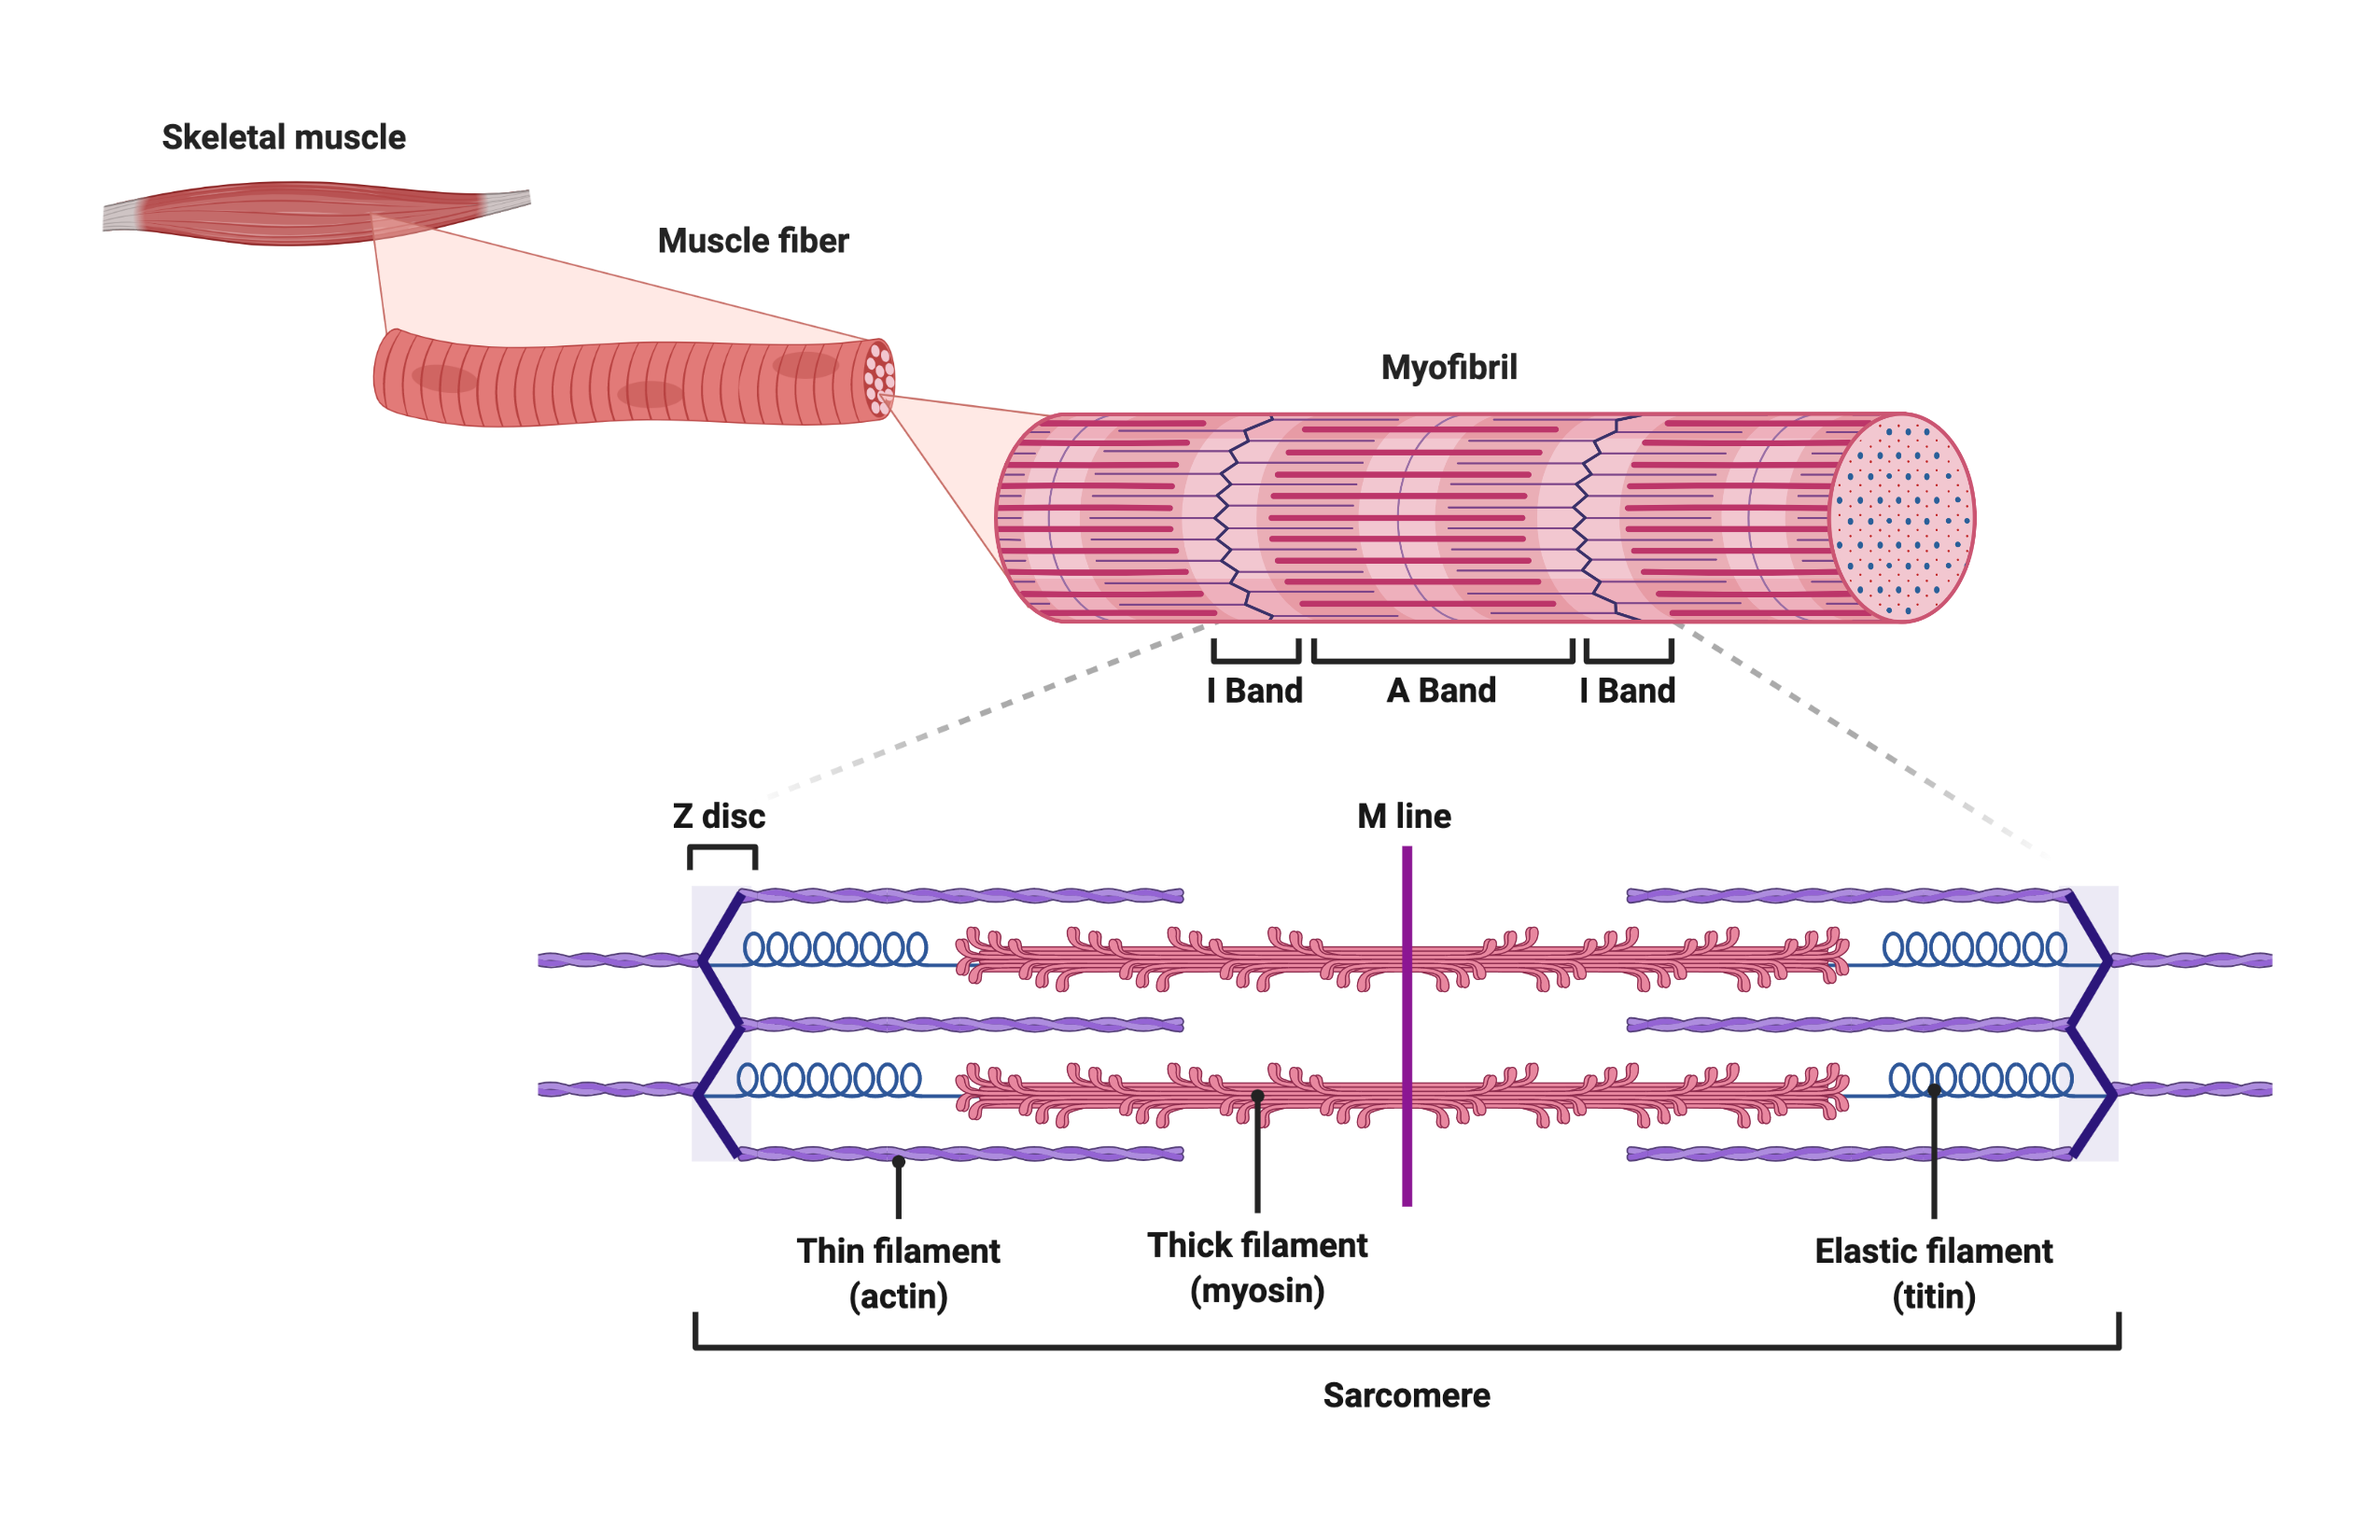
\includegraphics[width=1\linewidth]{./figure/Myofibril_Structure.png}
    \caption{Myofibril Structure \footnotesize{(Created with Biorender.com)}}
    \label{fig:Myofibril_Structure}
\end{figure}

\paragraph{Muscle Fibers} As can be seen in the hierarchical organization above and in Figure \ref{fig:Myofibril_Structure} muscle fibers include a set of myofibrils arranged in parallel. The boundary of a muscle fiber includes the endomysium and sarcolemma (cell membrane of the muscle fiber). Within the muscle fiber the myofibrils are surrounded by cellular components with critical roles to play to the the tensioning act. Components such as extensions of the sarcolemma terminating at sacroplasmic reticula which are critical during the process of excitation and regulation (covered in Chapters 3 and 4); the mitochrondria which are critical for energetics (covered in Chapter 5); and nuclei and associated protein manufacturing components such as the Golgi apparatus and ribosomes which are critical for Muscle Integrity (covered in Part III). For now we are focused on the muscle fiber components that generate tension. For the process of generating tension, the myofibrils are the functional building block of muscle fibers, and sarcomeres are the functional building blocks of a myofibril.



\subsection{Anatomy of a Sarcomere}
Figure \ref{fig:Sarcomere_Structure} also provides a detailed look at the tensioning proteins of the sarcomere that will be the focus of the rest of this chapter. The sarcomere includes all of the proteins between two Z-discs. These proteins are all actors in the act of passive tension (resistance to positive $\Delta$ length) and active tension through the cross-bridge cycle (sliding filament model).

\begin{figure}[!ht]
    \centering
    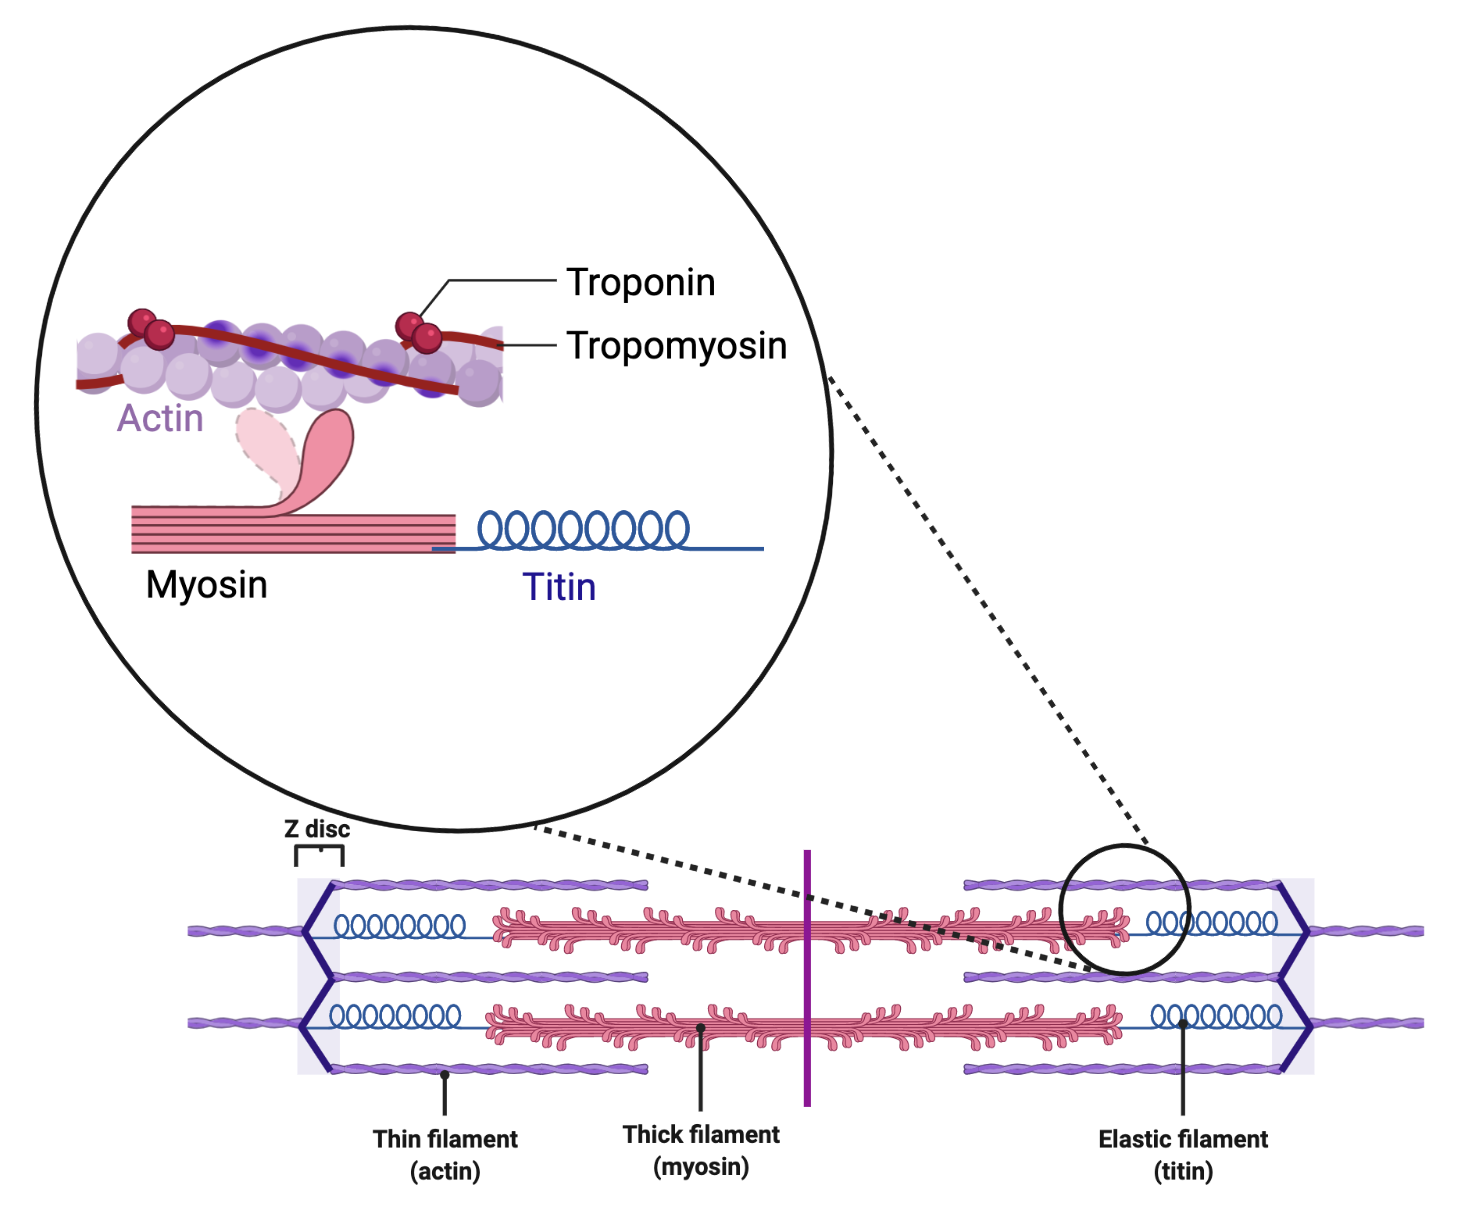
\includegraphics[width=1\linewidth]{./figure/Sarcomere_Structure.png}
    \caption{Sarcomere Structure: Primary Protein "Actors" \footnotesize{(Created with Biorender.com)}}
    \label{fig:Sarcomere_Structure}
\end{figure}

\paragraph{Primary Protein "Actors" and their Primary and Secondary Roles}
\begin{itemize}
\item Actin - primary role in active tension; secondary role in passive tension
\item Myosin - primary role in active tension; secondary role in passive tension
\item Troponin - Tropomyosin - primary role in active tension; secondary role in passive tension
\item Titin - primary role in passive tension; secondary role in passive tension
\end{itemize}

Passive tension is created when the Z-discs are pulled apart from one another. Active tension is created in an attempt to pull the Z-discs closer together. For our purposes knowing the precise structure of each of these proteins is not necessary,\footnotemark{}\footnotetext{As long as you recognize that their structure is of great importance. As with all proteins the structure is the foundation of function. Proteins form molecular machines that have very precise functions based on their very precise structure. Anything that alters the structure of a protein alters its function. Variations in pH and temperature that exceed certain boundary conditions, for example, have the capability of changing protein structure.} our focus is on the general structure of the proteins that allow the protein to play its role in tensioning. The arrangement of these proteins with one another within the sarcomere is important. For our purposes in this book everything you need to know about the structure and arrangement is based on the roles they play in the upcoming sections.

\subsection{Structure and Arrangement of the Sarcomere During Changes in Length}

The primary structural change to the sarcomere at different lengths is the distance between the Z-discs (Figure \ref{fig:Sarcomere_Lengths}). The majority of length changes in a muscle propagate down to, and emerge up from, changes in the distance between Z-discs of the sarcomeres.\footnotemark{}\footnotetext{The stress - strain relationships of tendons indicate that a tendon can experience about a 3\% change in length prior to damaging the tendon. This amounts to up to a 6\% change in muscle length when accounting for tendon at each of two attachments. Whether this contributes to a muscle change in length is very contextual. During lengthening it would depend on how much tension is being produced (stress on the tendon), and during shortening it would depend on how much lengthening occurred in the tendon prior to shortening since the tendons do not produce active tension.} Increasing the distance between Z-discs reduces the interaction space between the actin and myosin and, once at a certain length, starts to pull on the elastic structure of titin (unwinding of titin). Decreasing the distance between Z-discs will result in increasing the interaction space between actin and myosin, and recoil of titin to a point; followed by crowding of potential actin myosin crossbridges (decreasing interaction space), and compression of titin. The implications of these structural changes are discussed in the sections on Active and Passive Tension.

\begin{figure}[!ht]
    \centering
    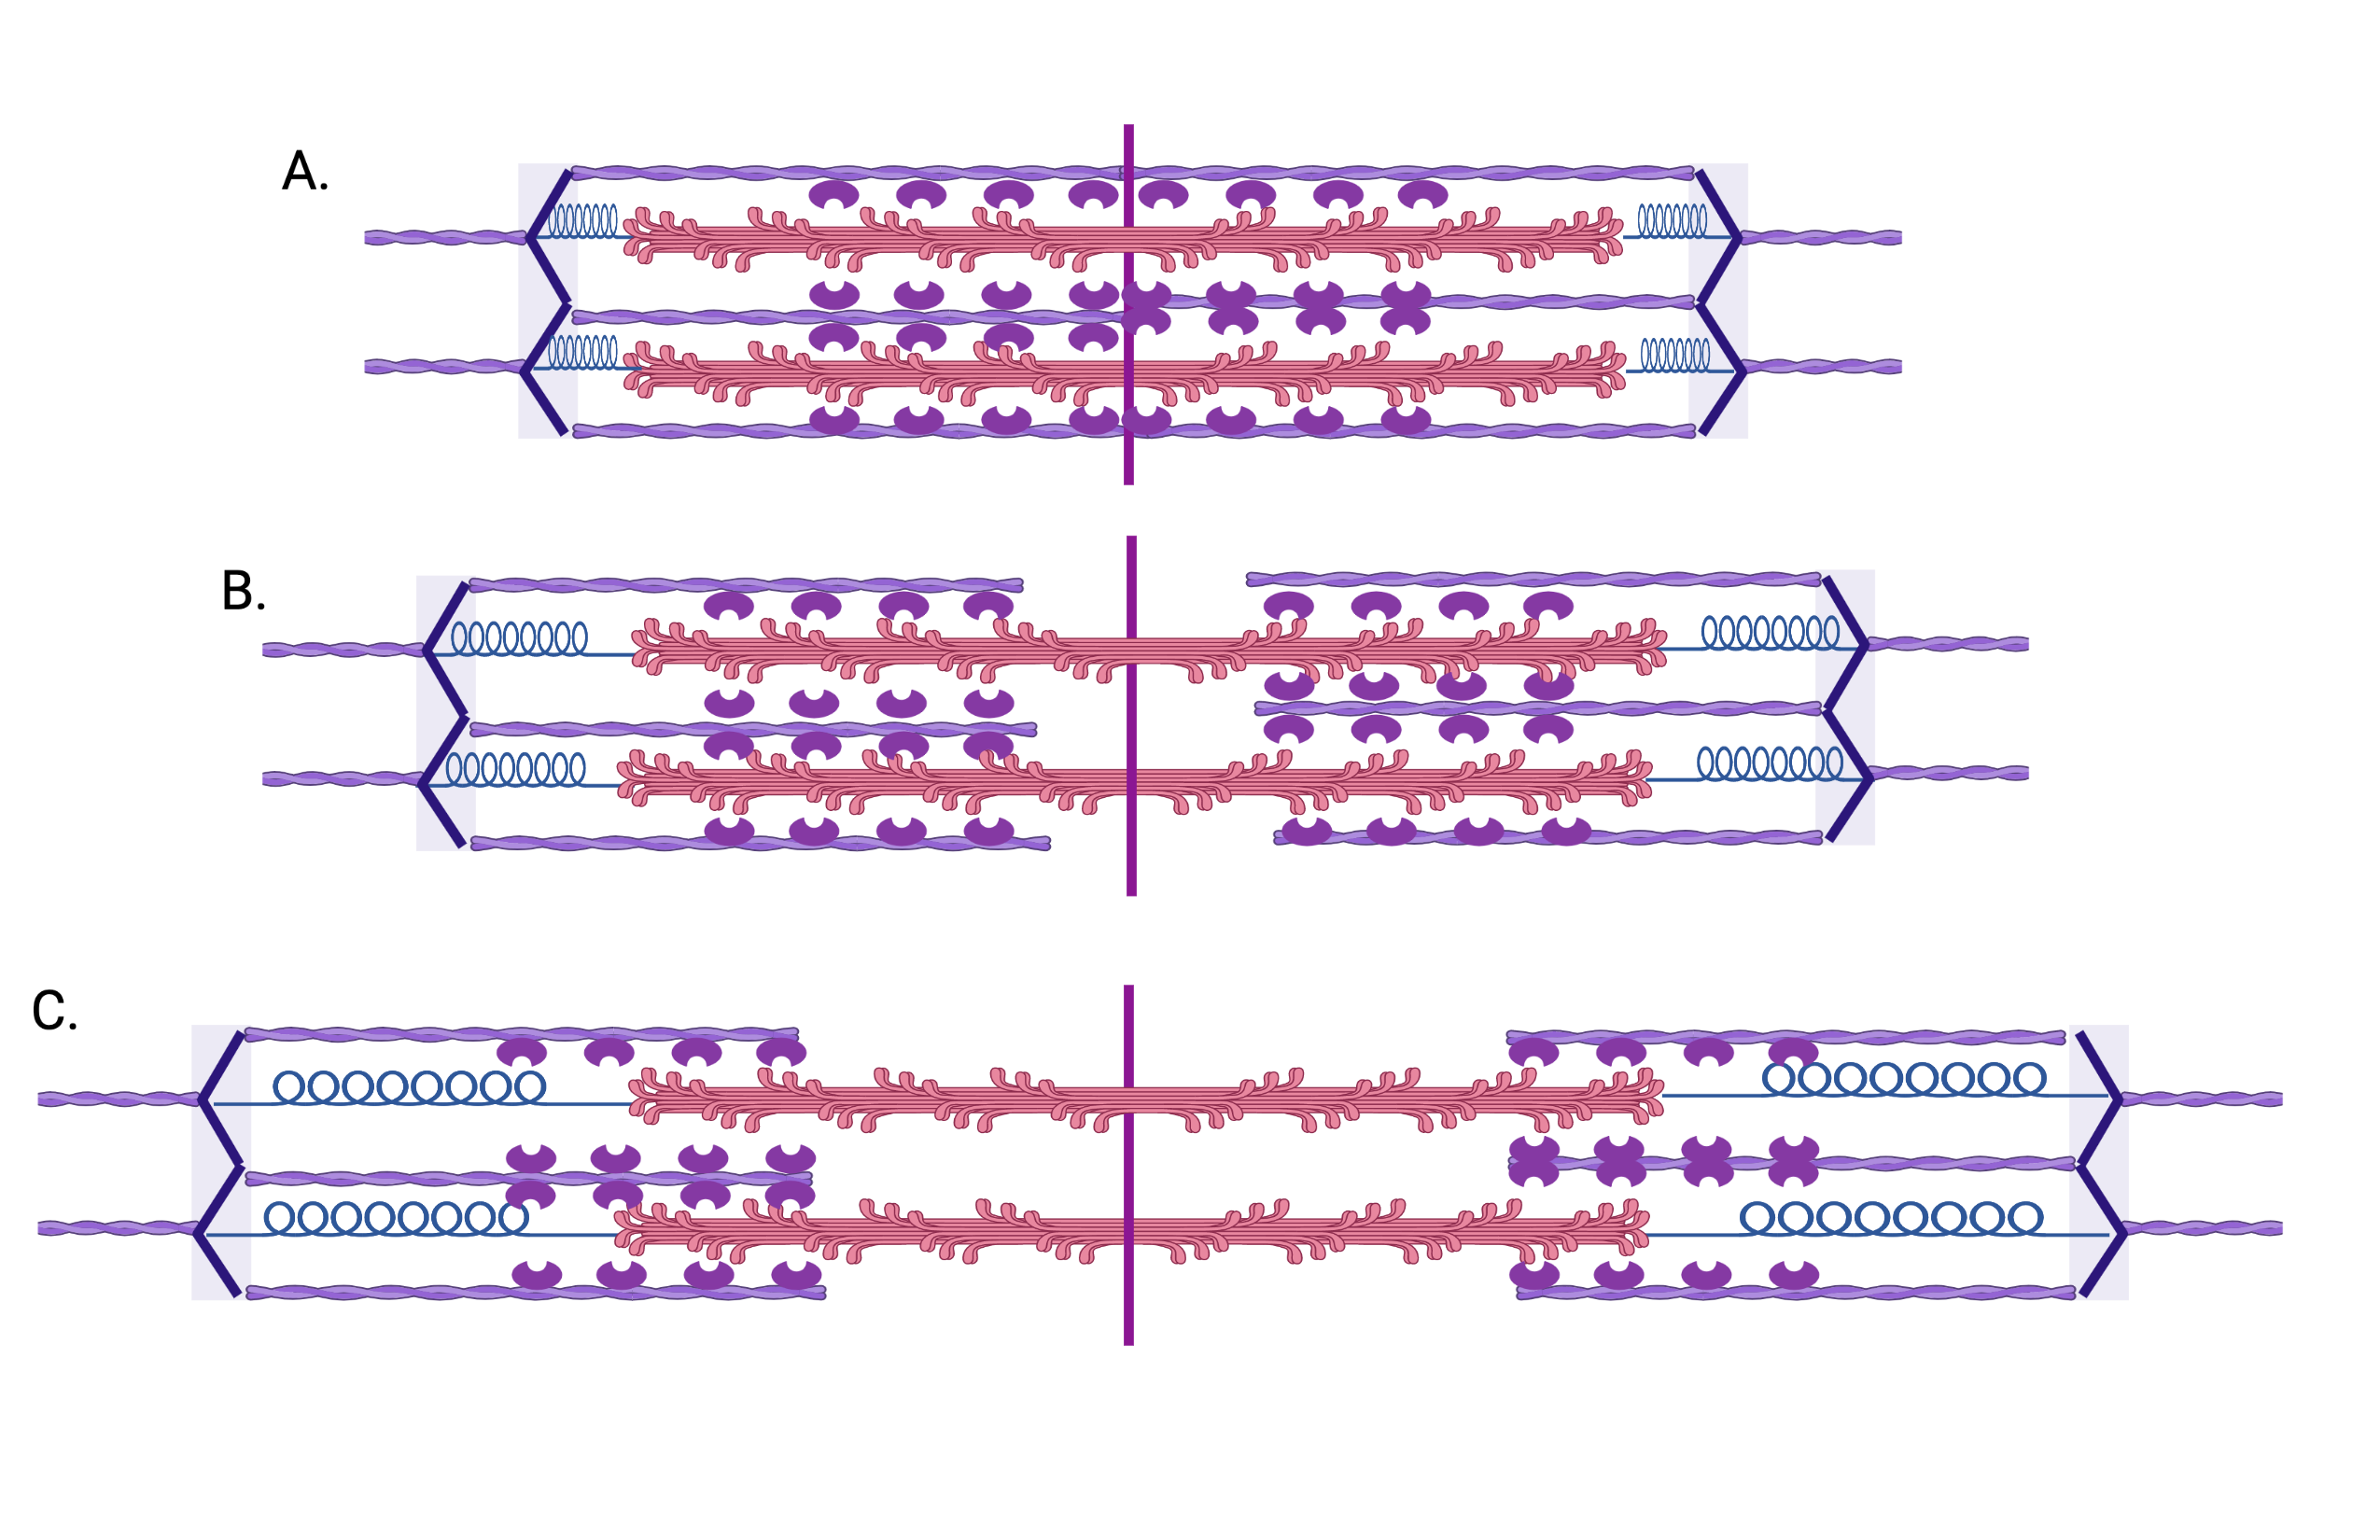
\includegraphics[width=1\linewidth]{./figure/Sarcomere_Lengths.png}
    \caption{Sarcomere Lengths. A. Shortened; B. Relaxed / resting; C. Lengthened \footnotesize{(Created with Biorender.com)}}
    \label{fig:Sarcomere_Lengths}
\end{figure}

\section{Passive Tension}
Passive tension is created when the Z-discs are pulled apart from one another. During positive $\Delta$ length the muscle fibers increase in length and the Z-discs of sarcomeres are pulled apart. The amount of passive tension developed (measured as force that resists lengthening) is a function of the relative length of the muscle this is primarily due to the relative length of titin. This relationship is the passive component of what is called the length - tension relationship (Figure \ref{fig:passive_lt}) (Figure \ref{fig:passive_lt}).

\begin{figure}[!ht]
    \centering
    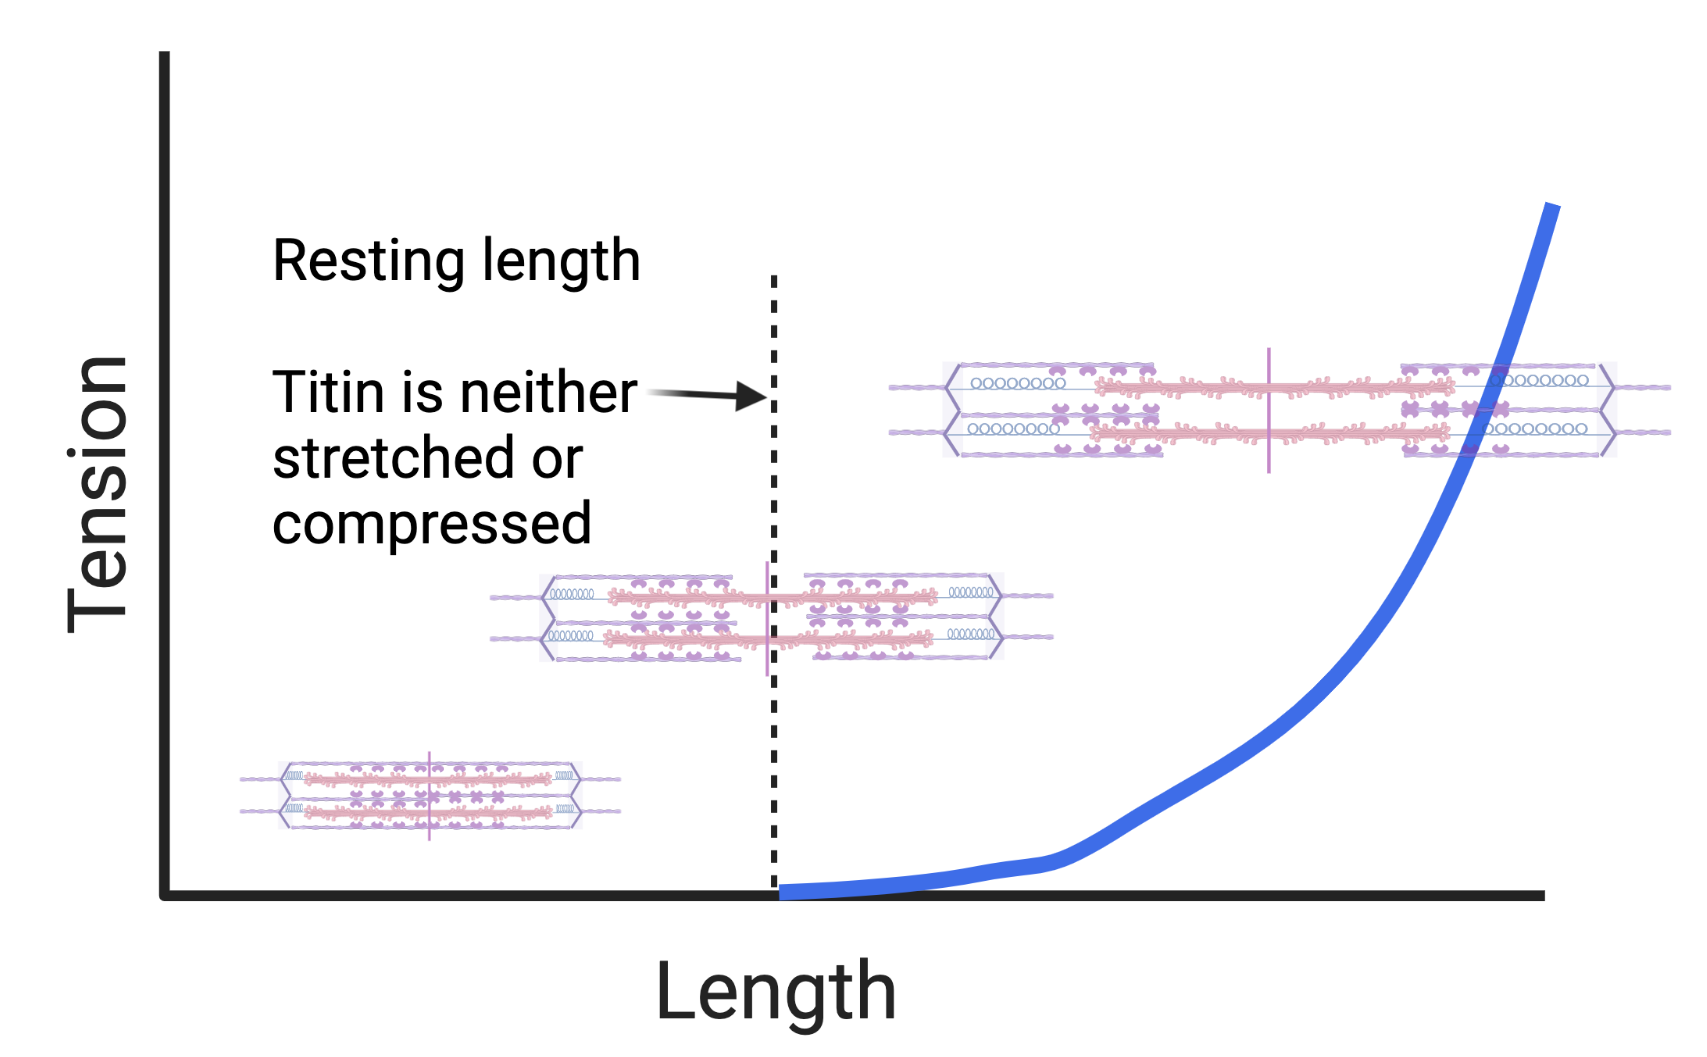
\includegraphics[width=1\linewidth]{./figure/passive_lt.png}
    \caption{Passive Component of the Length Tension Curve \footnotesize{(Created with Biorender.com)}}
    \label{fig:passive_lt}
\end{figure}

\paragraph{Muscle Tone}
At any given moment in the “inactivated” muscle there are some attachments between actin and myosin. The number of actin and myosin attachments influences the passive tension developed at various lengths. This is referred to as muscle tone. Muscle tone is the amount of tension in a muscle when it is not activated, that is when it is not creating active tension (and hence is essentially passive tension). Muscle tone is also dependent on the length of the sarcomere since that length influences the number of possible actin myosin attachments. While related to changes in length, the presence of these actin myosin attachments in an inactivated muscle is primarily related to the underlying reasons for the attachments and will be covered in later chapters. For now simply keep in mind that muscle tone is directly proportional to passive tension.

\subsection{Passive Tension Role In Movement}
Passive tension can have a fundamental role in movement, and alterations in passive tension can therefore have a fundamental role in altered movement (kinesiopathology). When passive tension is developed there is a force developed by the muscle undergoing passive tension that creates a torque across the joint formed by the bones the muscle attaches. For example, when the hamstrings are lengthened and generate passive tension, that passive tension starts to create a flexion torque at the knee. If the hamstrings are then activated (start to generate active tension) then the total tension created is the sum of the active and the passive tension, which together create the force that creates the flexion torque at the knee. Muscles involved in gait (walking) can cycle through periods of passive tension and then use that passive tension to supplement active tension. For example, during running the calf muscles are lengthened while the foot is on the ground which increases passive tension. When it is time for that foot to propel the body the torque produced by the calf muscles is a combination of passive and active tension. In this situation, additional passive tension reduces the need for active tension and thus increases muscle efficacy (less energy is required, and therefore the muscle can sustain tensioning for a longer period of time).

\section{Active Tension}

Active tension is created when the muscle fiber transforms the chemical energy stored in adenosine tri-phosphate (ATP) into mechanical energy that allows myosin to actively slides actin from one actin-myosin crossbridge to another. This process is activated at the level of the muscle fiber, but all of the events involved directly in this energy transformation occur in the sarcomere. The result is a tension that pulls (or attempts to pull) the Z-discs of the sarcomere closer together.

\subsection{Sliding Filament Model}
The sliding filament model of active tension (also referred to as the sliding filament theory of muscle contraction) is well understood at the level we need to understand it.\footnotemark{}\footnotetext{There remains active investigation into the sliding filament process and the details of crossbridge kinetics. All models are wrong, some models are useful. The intricacy of events in reality is likely more complicated than represented by this model. The intricacy, combined with how quickly they occur, makes a complete understanding challenging. But what we know about it is useful for our purposes. We use this model to explain many phenomenon throughout the book.} 
\paragraph{}
Figure \ref{fig:Sliding_Filament} depicts the steps in the process of creating active tension. The steps are also enumerated below.

\begin{figure}[!ht]
    \centering
    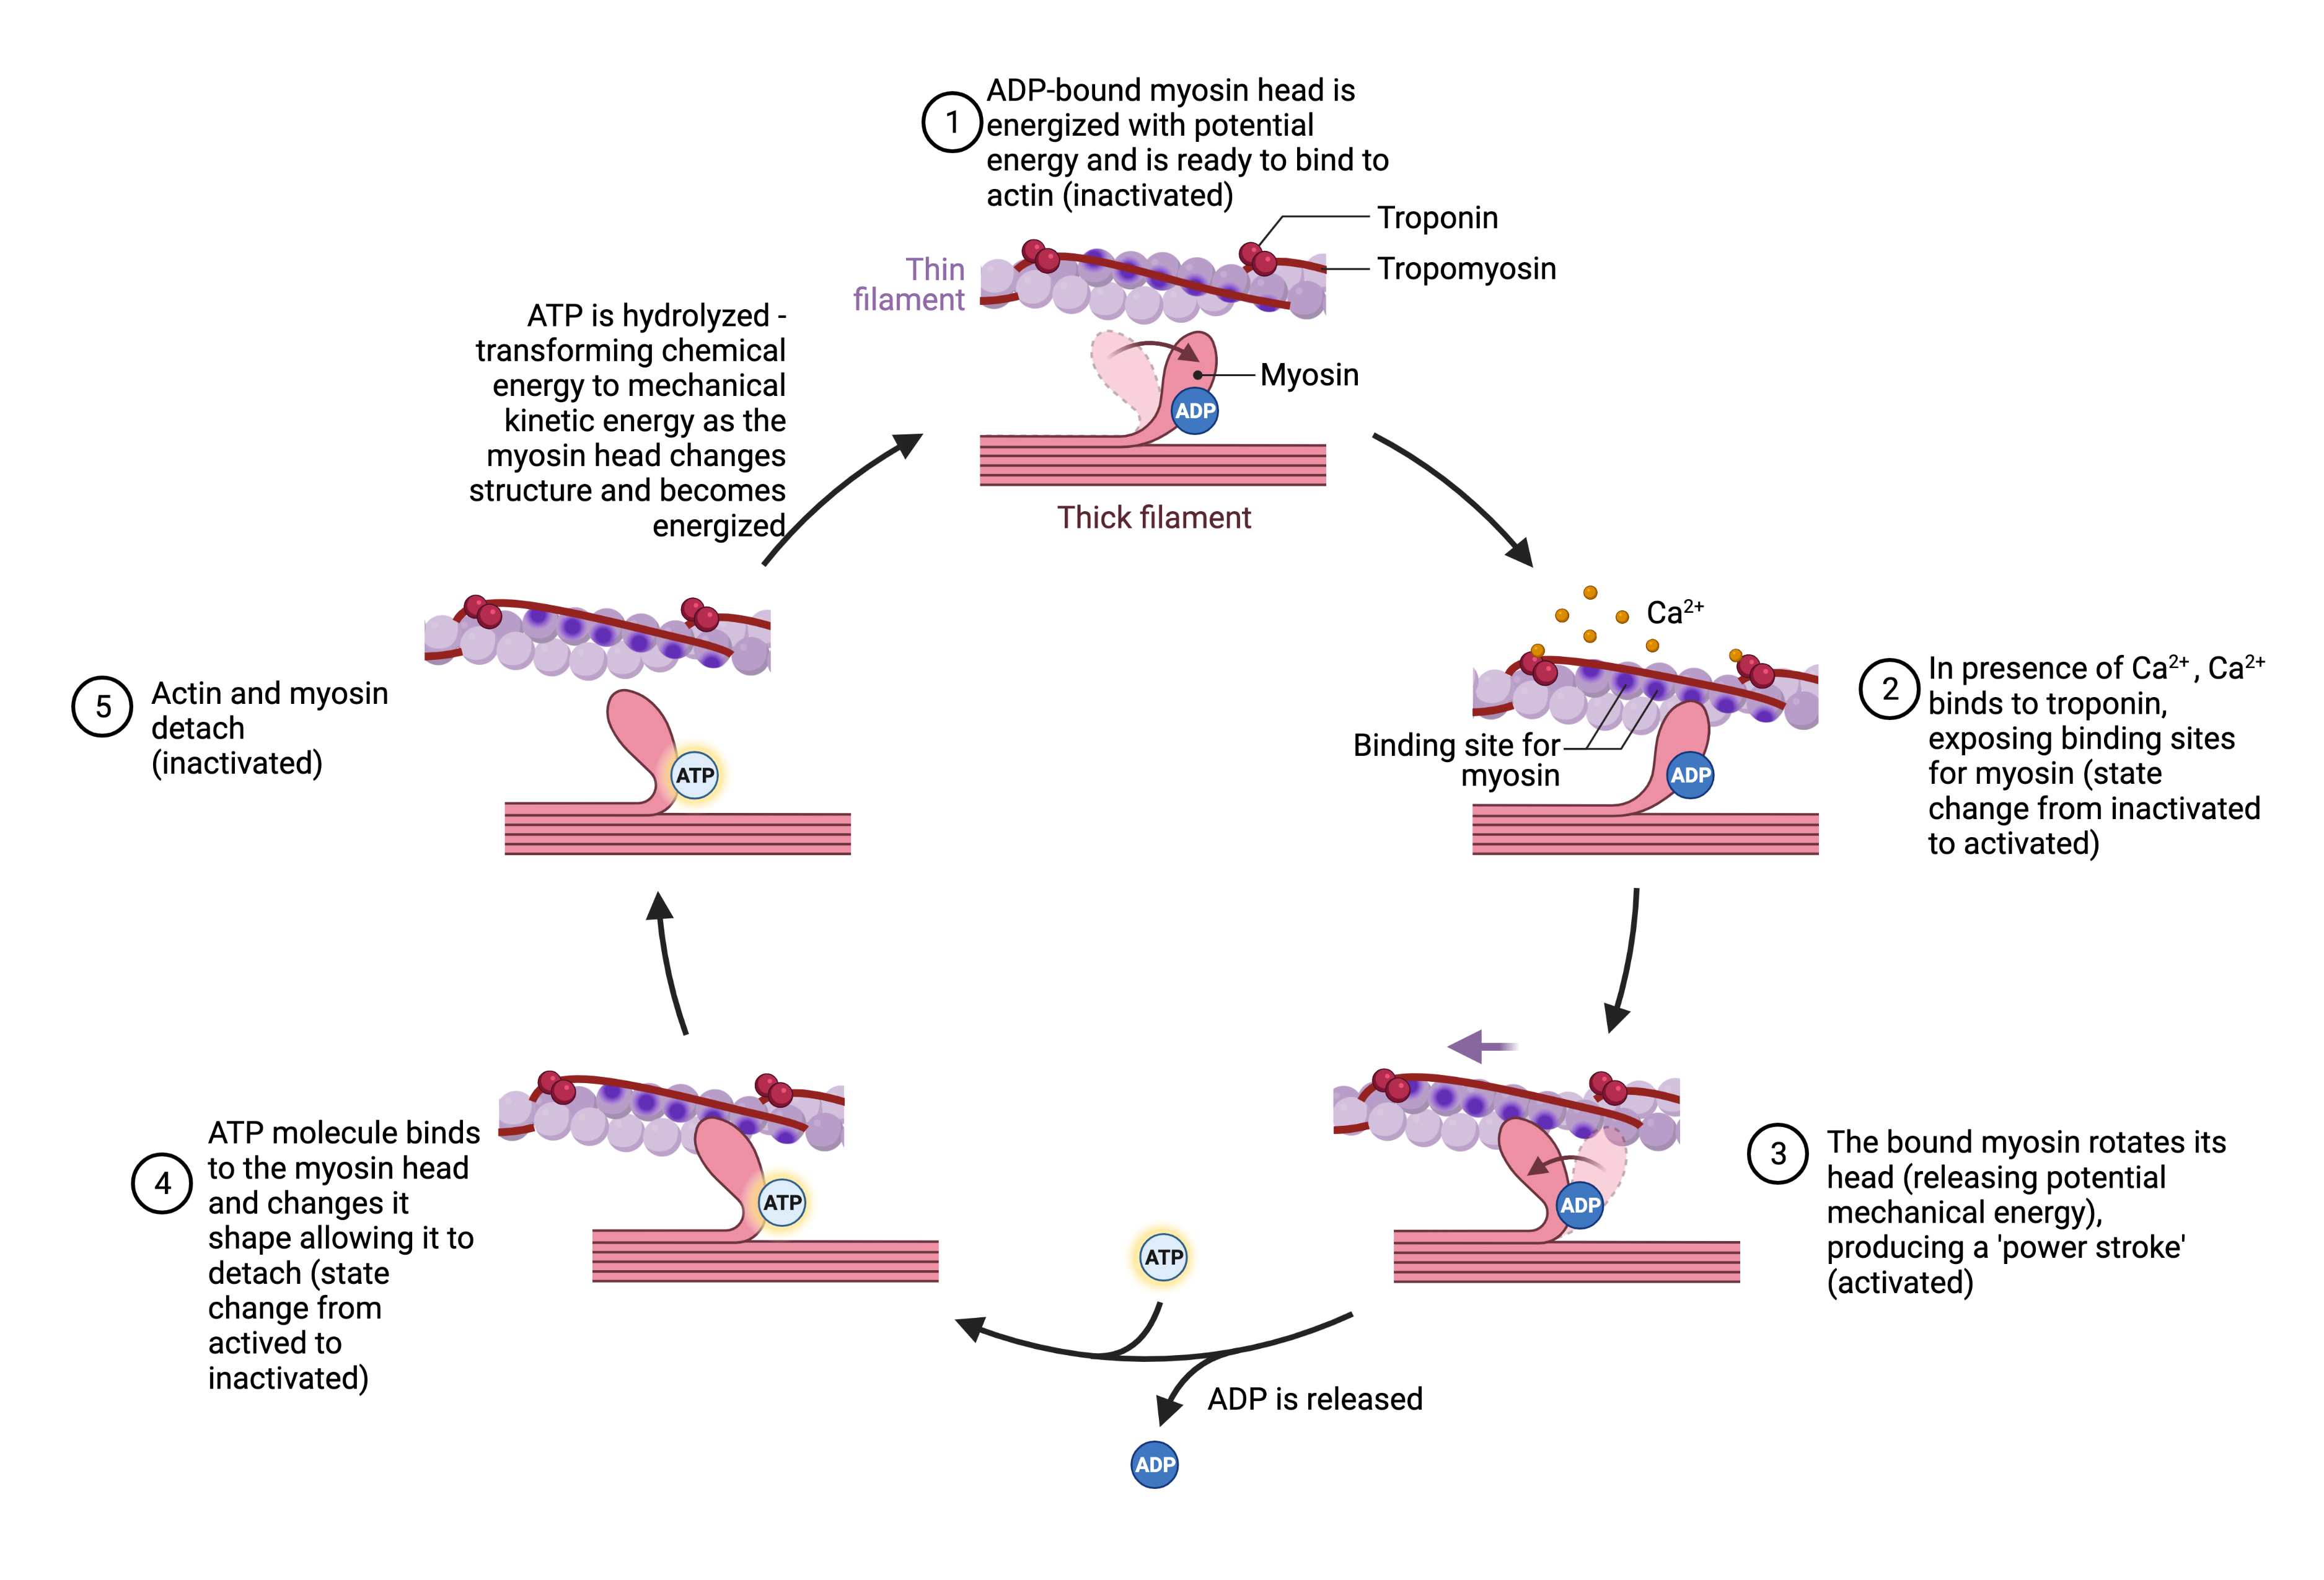
\includegraphics[width=1\linewidth]{./figure/Sliding_Filament.png}
    \caption{Sliding Filament Model of Active Tension \footnotesize{(Created with Biorender.com)}}
    \label{fig:Sliding_Filament}
\end{figure}

\begin{enumerate}
\item ADP-bound myosin head is energized with potential energy (from the release of a phosphate from ATP) and is ready to bind to actin. While the myosin head is energized, it is inactivated.
\item In the presence of calcium, calcium binds to troponin, moving tropomyosin and exposing actin binding sites. In crossbridge kinetics terminology this is the change in state of the crossbridge from inactivated to activated.
\item The bound myosin rotates its head (releasing potential mechanical energy), producing a 'power stroke'. The crossbridge remains activated.
\item ATP molecule binds to the myosin head and changes its shape allowing it to detach from actin (state change from activated to inactivated).
\item Actin and myosin are detached and not energized (inactivated)
\end{enumerate}

\subsubsection{Crossbridge Kinetics}
The current understanding of the molecular basis for muscle contraction comes from Huxley’s (1957) kinetic model of the cyclic interaction between actin myosin crossbridges \cite{huxley_muscle_1957}. Active tension behavior of a sarcomere (such as the force - velocity relationship described below) does not originate from the behavior of individual crossbridges, but from the collective action of all activated crossbridges in the sarcomere as they asynchronously go through the energy (ATP) dependent cycle described in the sliding filament model. In the crossbridge kinetics model the sarcomere has, at any given length, a number of possible crossbridges.  The number of possible crossbridges is the crossbridge interaction space. Each possible crossbridge has two states, activated and inactivated. The active tension of a sarcomere is directly proportional to the number of crossbridges in the activated state which is influenced by both the concentration of calcium in the sarcomere and the length of the sarcomere. The sliding filament model describes one cycle of crossbridge kinetics (one cycle of inactivation to activation to inactivation).

\paragraph{Introduction to Twitch}
A twitch is the fundamental unit of active tension. It is a spike in active tension generated when crossbridges are activated from one excitation of a muscle fiber. A twitch can be considered at the level of the sarcomere, myofibril, fiber and muscle. A twitch \textit{in situ} is perceptible but not functional. If many muscle fibers twitch at the same time it may be experienced as a spasm, though not long lasting. Sustained spasms (myotonia) involve more than a twitch. A twitch can be thought to equate to one cycle of crossbridge kinetics. The force of a twitch is directly proportional to the number of crossbridges in the activated state, meaning if there are more crossbridges cycling into the activated state there is more tension. Experimentally, all sarcomere twitches will tend to produce the same tension when performed at the same length and when separated by enough time. A myofibril twitches can have small variations in tension depending on how many of its sarcomeres have crossbridge cycling from the stimulus provided. Muscle fiber twitches can vary greatly in the amount of tension during a twitch because there is greater potential for variation in the number of sarcomeres involved in crossbridge cycling. Experimentally the number of sarcomeres involved in cross bridge cycling will depend on the amount of excitation stimulus provided. 

\paragraph{Introduction to Tetany}
When a sarcomere is repeatedly excited the resultant twitches (spikes in tension) from each excitation start to fuse with each other and the spikes in tension from each twitch get smooth while the overall tension increases. This transition to a smooth rise and even maintenance of tension from a sarcomere is tetany. The greater the number of excitations the greater the tension developed in tetany because the result is a greater number of crossbridges in the activated state at any given moment across time. The amount of tension developed reflects the ability to attain tension, and the period of time tetany can last during repeated excitations is the ability to sustain tension.
In Chapter \ref{chp:excitation} the concepts of twitch and tetany are the bridge between muscle excitation and crossbridge kinetics. In Chapter \ref{chp:regulation}they are used to connect muscle regulation to excitation. 

\subsection{Active Component of the Length Tension Relationship}
Since the sarcomere crossbridge interaction space varies with its length \footnotemark{}\footnotetext{Distance between the Z-discs} the number of activated crossbridges also varies with its length. Therefore, under conditions of maximal activation (high calcium concentrations), the active tension varies with sarcomere length.  The crossbridge interaction space decreases as the distance between the Z-discs increases or decreases from an ideal distance. In a circular we then define the ideal distance between the Z-discs (sarcomere length) as the length that maximizes the crossbridge interaction space. 

The active component of the length tension relationship was originally measured using isolated muscle fibers under isometric conditions at different lengths. However, we do tend to consider the impact of the underlying phenomenon during activation that includes dynamic changes in length. As the distance between the Z-discs decreases, such as during negative $\Delta$ length (concentric) or when muscle activation begins while in a shortened length, the actin-myosin interaction space is decreased because of the actin binding sites increase in concentration with a limited number of myosin heads (near the M-line) which reduces the number of potential crossbridge sites. This reduces the active tension. As the distance between the Z-discs increases, such as during positive $\Delta$ length (eccentric) or when muscle activation begins while in a lengthened length, the actin-myosin interaction space is decreased because parts of actin are not in proximity with myosin which reduces the number of crossbridge sites. This reduces the active tension.

The active component of the length tension relationship is depicted in Figure \ref{fig:active_lt}.\footnotemark{}\footnotetext{The depiction of the actin myosin crossbridges in this particular rendering includes overlap of the actin during the shortened range. Whether there is such overlap vs. crowding of sites near the M-line is still an open discussion, or at least as far as the author is aware. It's another example that all models are wrong and some models are useful.}

\begin{figure}[!ht]
    \centering
    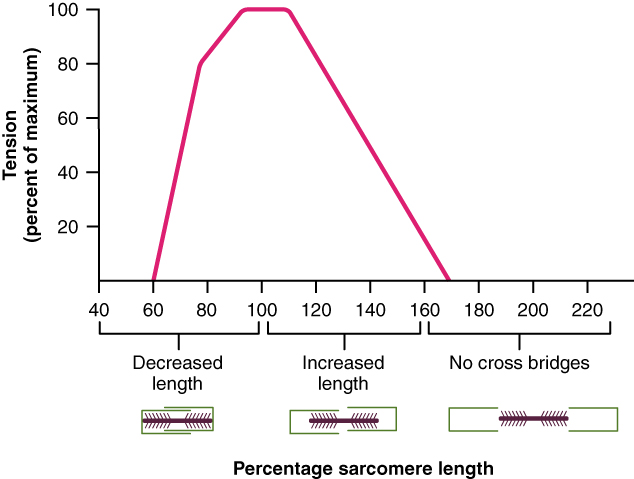
\includegraphics[width=1\linewidth]{./figure/active_lt.jpg}
    \caption{Active Component of the Length Tension Curve \footnotesize{(OpenStax, CC BY 4.0, \href{https://creativecommons.org/licenses/by/4.0}{via Wikimedia Commons})}}
    \label{fig:active_lt}
\end{figure}


\subsection{Length-Tension Relationship (Active \& Passive Components)}

The full length tension relationship of a sarcomere, and a myofibril, is depicted in Figure \ref{fig:lt}. It is important to keep in mind that this relationship is based on experiments of myofibrils removed from their anatomical locations and maximally activated under isometric (zero $\Delta$ length) conditions. The length tension relationship of any particular muscle \textit{in situ} may vary from this general relationship based on a number of factors such as the normal resting position of the muscle with anatomical attachments, the pennation arrangement, whether the conditions of maximal activation are met (rarely), whether the conditions of zero $\Delta$ velocity is met (rarely during functional movement), or whether the muscle crosses more than one joint. Two of these deserve special mention. 

\begin{figure}[!ht]
    \centering
    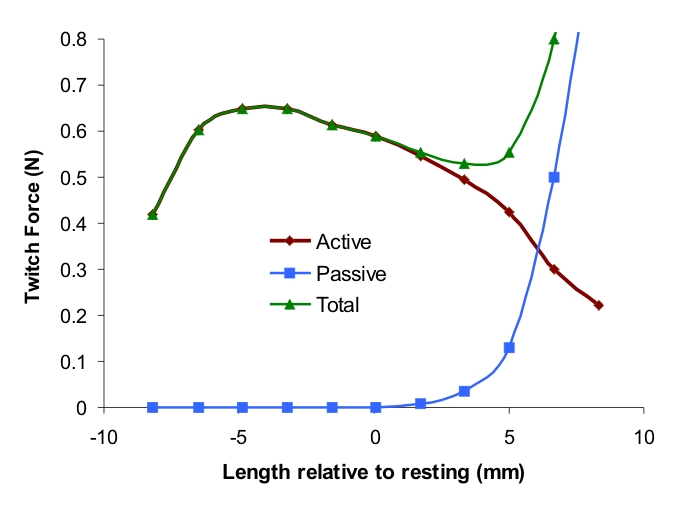
\includegraphics[width=1\linewidth]{./figure/lt.jpg}
    \caption{Full Length Tension Curve with Total Tension \footnotesize{(Public Domain figure from \href{https://commons.wikimedia.org/wiki/File:Lengthtension.jpg}{Wikimedia Commons})}}
    \label{fig:lt}
\end{figure}


\paragraph{Manual Muscle Testing} During manual muscle testing (MMT) physical therapists are taught about the ideal joint range of motion (ROM) for testing. These ROMs are typically positions that put the muscle at a length intended to maximize tension based on the active component of the length tension relationship. 

\paragraph{Active \& Passive Insufficiency & Sufficiency}
A special situation that arises in muscles that have attachments crossing more than one joint is that the ROM of both joints influences the muscle length. Since muscle length influences both active and passive tension the position or movement of both joints influences active and passive tension.
Active insufficiency occurs when the active tension a muscle creates is impacted by the position or movement of the joints (at least 2) that is crosses. For example, if you attempt to extend the hip and flex the knee at the same time using active tension your ability to generate active tension will decline quickly due to the fact that the hamstring sarcomere Z-discs are getting closer and actin-myosin interaction space is decreasing.
Passive insufficiency occurs when the passive tension a muscle creates is impacted by the position or movement of the joints (at least 2) that it crosses. For example, if you attempt to flex the hip and extend the knee at the time time, passive tension develops due to the hamstring sarcomere Z-discs getting further apart and titin is resisting further changes to its length.\footnotemark{}\footnotetext{Please note that the focus here on titin is for simplicity. Other connective tissues within the muscle contribute to this passive tension. It is also possible that extra-muscular connective tissue such as fascia can contribute to the passive tension developed during passive insufficiency since these movements tend to not serve critical movement functions. They tend to be movements contrary to what would be considered critical movement functions.}
Active and passive sufficiency is the principle (possibly new to this book) that most functional movements tend to avoid active and passive insufficiency. Most functional movements tend to use multi-joint muscles in a way that optimize their tension generating capabilities based on the length tension relationship. For example, during squatting and climbing, the hamstring sarcomere length does not change much since these movements couple hip flexion with knee flexion (one direction of movement), and hip extension with knee extension (the other direction of movement).

\subsection{Necessary Molecules}
Most of the molecules involved in the sliding filament model are protein actors in the sarcomere. However, there are two molecules that make important appearances and deserve special mention at this point as a preface to where we are heading as we progress toward connecting muscle physiology to clinical physiology.

\paragraph{} 
Calcium($Ca^{2+}$) enters the scene to get things started. It triggers the events that lead to the crossbridge state change from inactivated to activated. It is the signaling molecule utilized to activate the process of the sliding filaments for active tension. It is stored in an organelle in close proximity to the sarcolemma called the sarcoplasmic reticulum. $Ca^{2+}$ enters the cell once the sarcolemma and sarcoplasmic reticulum is excited and is an important part of Chapter 3 on Excitation. Calcium is the connecting molecule in the process called “excitation - contraction coupling” which we call “excitation - activation coupling”. As you can imagine, having sufficient $Ca^{2+}$ available for the muscle fiber is essential. The processes supporting sufficient $Ca^{2+}$ concentrations is covered in Part II: Muscle Support and involves the neuroendocrine and gastrointestinal systems. 

\paragraph{}
ATP provides the chemical energy that is transformed into mechanical energy by the molecular motors within the sarcomere. ATP is kept in limited quantities inside the muscle cell. It is used to energize cellular processes that require energy (do not confuse cellular processes with chemical reactions). Examples of cellular process include transcription and translation or a pump that moves ions across a membrane to form a gradient. Chemical reactions are transformations that proceed bidirectionally with one direction usually favored by mass balance and enzyme catalysts. Since ATP is stored in limited quantities (enough for seconds of myosin energizing), the muscle fiber must be able to convert other forms of energy (usually chemical energy) into ATP. That is the primary topic of Chapter 5 on Muscle Energetics.


\section{Force \& Velocity}

Throughout the next few chapters we develop an understanding of force (as the result of tension) and velocity. Our understanding of the relationship between them will develop from two perspectives: the Force - Velocity (FV) and the Velocity - Force (VF) Relationships. In this chapter we introduce the concept and these two perspectives (FV \& VF), and consider what our current understanding about sarcomeres contributes to that understanding.

By force we are referring to force being measured that is the result of muscle tension (total tension). By velocity we are referring to changes in length over time. $\Delta$ length and velocity are related: 

\begin{equation} \label{eq_velocity}
velocity \ = \frac{\Delta \ length}{time}
\end{equation}

 Once we consider velocity we are considering changes in length, which makes the force velocity relationships different from length-tension relationships. Length tension relationships are experimentally observed under conditions of isometric (zero $\Delta$ length) conditions and is theoretically extended to dynamic (non zero $\Delta$ length) conditions. Force velocity relationships must be experimentally observed under dynamic (non zero $\Delta$ length) conditions. Since velocity involves changes in length, the force velocity relationships must include considerations related to the implications of the length tension relationship. Even though the length tension relationship is observed under conditions of isometric activation, what the length tension relationship represents (changes in sarcomere structure that result in changes in passive elastic and active tension) is occurring during a change in sarcomere length.

\paragraph{Movement Energetic Perspective}
Before proceeding with the FV and VF relationships it is important to point out that these relationships can be differentiated from a third perspective - the movement energetic perspective. Keeping in mind that movements are the sum of torques acting across joints with a larger imbalance between torques produce a “faster” movement, and keeping in mind that torques are generated by force which is generated by active muscle tension, and that active muscle tension is proportional to the number of activated crossbridges, and that the number of activated crossbridges is proportional to the amount of ATP being utilized, we can conclude that “faster” movements utilize more ATP (that is, they are more energetic). The movement energetic perspective is discussed in Chapter 5 on Muscle Energetics. In summary, it is why running at a faster pace makes you breath heavier than a slower pace; and why certain running paces (sprinting) are not possible for very long. \footnotemark{}\footnotetext{We are keeping the movement energetic perspective separate from the FV and VF relationships because it is not traditionally considered when discussing these relationships.} 

\subsection{Sarcomere Arrangement}

The FV and VF relationships can be considered at the level of the sarcomere, myofibril, muscle fiber or whole muscle. It is useful to review the arrangement of the sarcomeres across this hierarchy since the force generated and the velocity of shortening are both related to whether sarcomeres are arranged serially or in parallel. Tension within a sarcomere is transmitted to the myofibril, and sarcomeres in a myofibril are arranged serially.  Myofibrils are arranged in parallel (some may be serial)in a muscle fiber. And muscle fibers are arranged in parallel (some may be serial) within a muscle fascicle. And muscle fascicles are arranged in parallel within the muscle.

\paragraph{Sarcomeres in series - higher maximal velocity} 

A myofibril consists of sarcomeres arranged in series. As explained in Chapter 1 on Fundamentals, this means the change in length of a myofibril is the sum of  the change in length of the sarcomeres. Increasing the number of sarcomeres in a myofibril does not change the amount of tension that can be created since they are in series and this does not change the cross sectional area. Therefore, a myobril with more sarcomeres serially connected (longer) can achieve higher maximal velocity of shortening. If a sarcomere can shorten $1 \mu m$ in a millisecond, then a myofibril of 1000 sarcomeres shortens 1 mm and a myofibril of 500 sarcomeres shortens at 0.5 mm in 1 microsecond.


\paragraph{Sarcomeres in parallel - higher maximal force}
A muscle fiber consists of myofibrils arranged in series and in parallel. This means that the change of length of the muscle fiber is proportional to the change of length of myofibrils in series (which is proportional to the number of sarcomeres organized in series). Myofibrils are also arranged in parallel. The number of myofibrils in parallel influence the cross sectional area of the muscle. The tension generated increases proportionally with the cross sectional area of the muscle which can be achieved by increasing the number of myofibrils, and thus sarcomeres, in parallel. If a sarcomere generates 1 unit of tension then 10 sarcomeres serially connected also create one unit of tension (See Figure \ref{fig:Sacromeres_series_parrallel}. However, if those 10 sarcomeres are connected in parallel then they will together create 10 units of tension.

\subsection{Force - Velocity \& Velocity - Force Relationships}

\paragraph{Velocity - Force Relationship}
We consider the VF Relationship under the condition of no resistance. In the VF relationship force is a function of velocity. The muscle is not resisted \footnotemark\footnotetext{By anything of any significance beyond the resistance of joint friction, limb mass and air resistance. The point is that, in this situation, velocity is not impacted by the necessity for the muscle to generate enough active tension to overcome the force of the resistance.} and we consider the force that can be achieved with varying levels of velocity. We plot the independent (manipulated) variable on the X axis, and as the dependent (observed) variable we plot force on the Y axis. We consider the VF relationship in Chapter 4 on Muscle Regulation since the phenomenon involves variations in muscle fiber types (heterogeneity between muscle fibers).

\paragraph{Force - Velocity Relationship}
We consider the FV Relationship under the condition of resistance. In the FV relationship velocity is a function of force. The relationship between force and shortening velocity is visualized by plotting the velocity of a shortening muscle as a function of the load (or force) pulling on the muscle \cite{seow_molecular_2022}. The muscle is resisted and we consider the velocity that can be achieved with varying levels of resisted muscle force. We plot the independent (manipulated) variable on the X axis, and the dependent (observed) variable velocity on the Y axis. FV has an inversely proportional hyperbolic relationship and was first described by Hill \cite{seow_hills_2013}. Because power is the product of force and velocity it has a parabolic relationship which achieves its peak at neither the extreme of velocity or force \cite{seow_hills_2013}. 

\subsubsection{Force Velocity Relationship during Shortening (Concentric)}
Figure \ref{fig:fv_shortening_1} shows the FV relationship during concentric (shortening) activation with power. It is a consistent finding that peak power occurs between 20 and 30\% of peak force.

\begin{figure}[!ht]
    \centering
    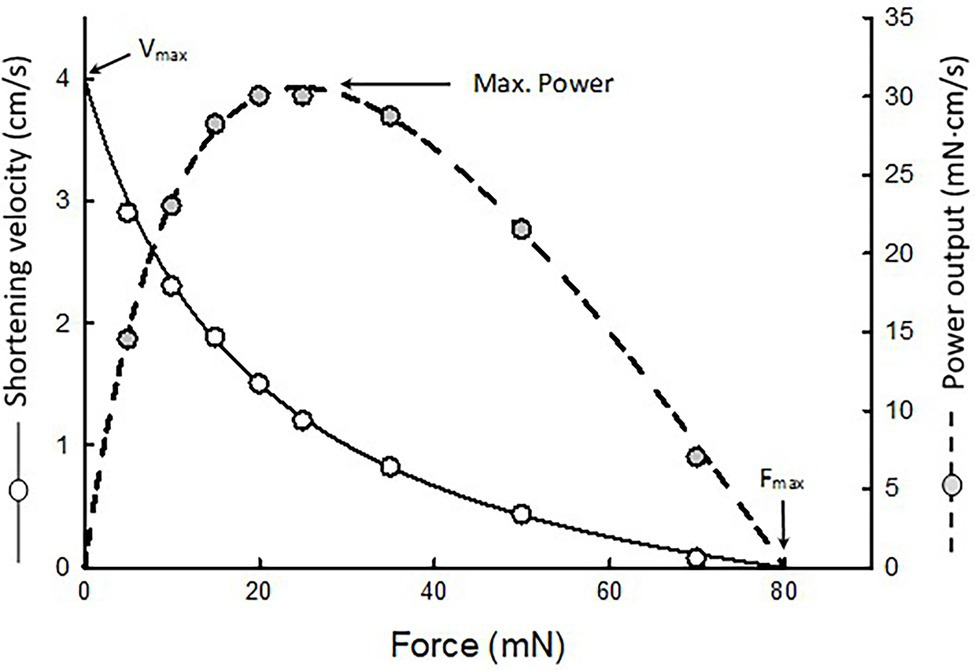
\includegraphics[width=1\linewidth]{./figure/fv_shortening_1.jpg}
    \caption{Force Velocity Curve and Power Relationship during Shortening \footnotesize{Creative Commons Attribution License (CC BY) Figure from \cite{seow_hills_2013}}}
    \label{fig:fv_shortening_1}
\end{figure}

Figure \ref{fig:fv_shortening_2} includes five FV and power curves to demonstrate the impact of sarcomere arrangement. Readers should familiarize themselves with the various curves and make sure they understand how they relate to sarcomere arrangement.

\begin{figure}[!ht]
    \centering
    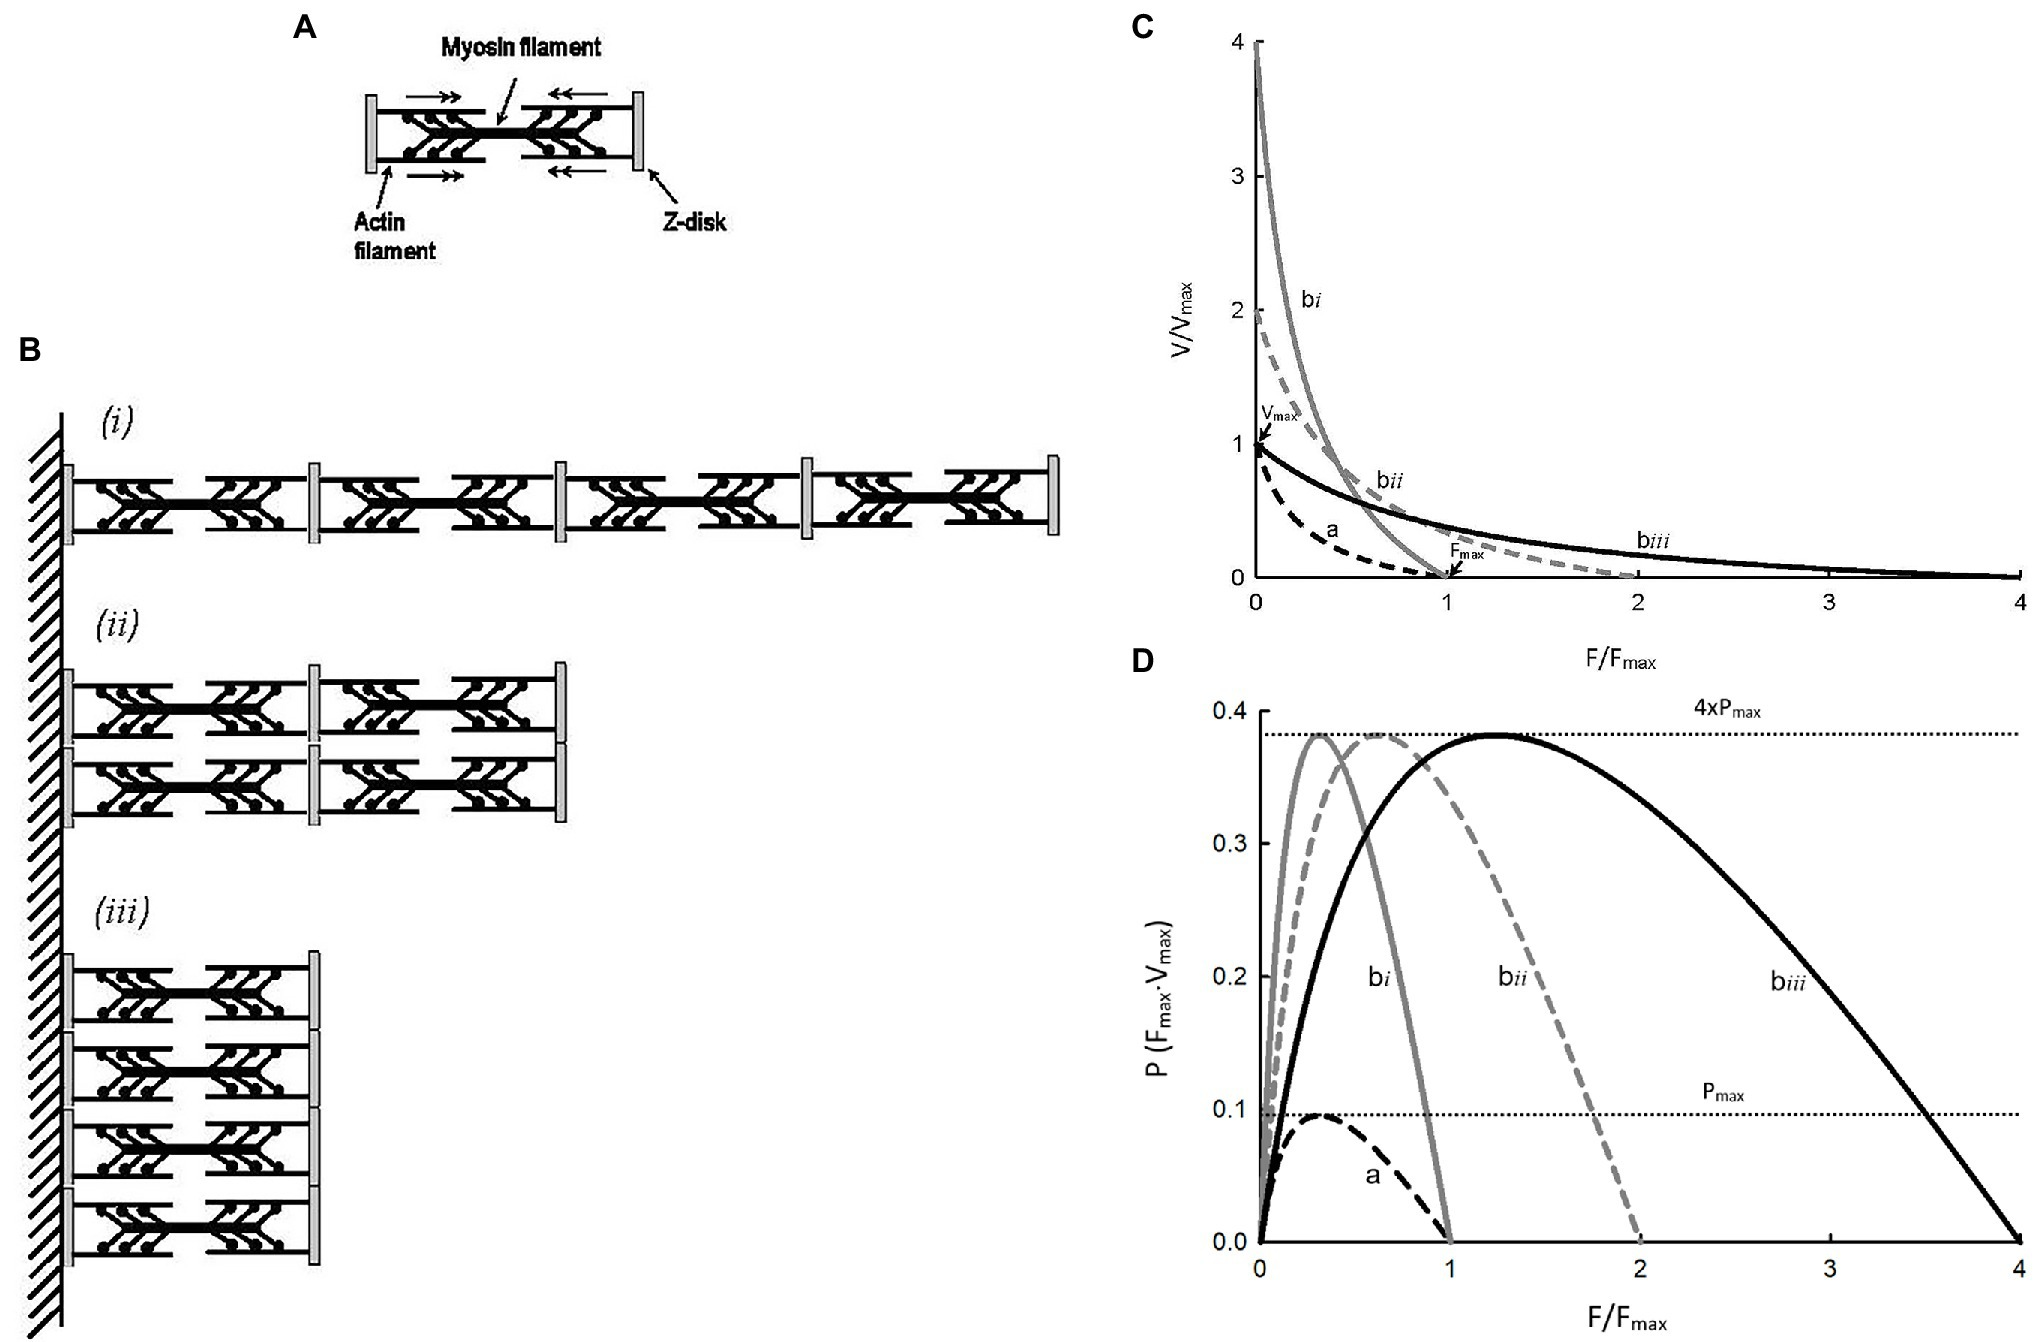
\includegraphics[width=1\linewidth]{./figure/fv_shortening_2.jpg}
    \caption{Impact of Sarcomere Arrangement on the FV Relationship during Shortening. \footnotesize{Creative Commons Attribution License (CC BY) Figure from \cite{seow_molecular_2022}}}
    \label{fig:fv_shortening_2}
\end{figure}

\paragraph{}
There are two factors contributing to the FV relationship during concentric activation. First, is the fact that a concentric activation requires the muscle generate more torque than the resistance (load). When someone generates just enough torque, they generate a minimal (non zero) velocity. As load is reduced, the maximal active tension of the muscle creates an abundance of torque and this results in greater velocity. 

Second, under the condition of attempting to move as fast as possible, as the load on and the force generated by a muscle increases, there is an increase in the velocity. The drop in force is due to the drop in load, which then allows for a higher velocity. However, it is also true that at the higher velocity there is a lower capability for generating force (the VF relationship). This is due to two factors that we can trace back to crossbridge kinetics. A, with increased velocity of shortening the crossbridge interaction space decreases rapidly which brings the sarcomeres into a shorter length and reduces the tension they can create (i.e. length tension relationship). B, with increased velocity of changes in length there is less time for crossbridges to be in their activated state, which means at any moment there is a lower number of possible crossbridges in the activated state. 

\paragraph{Experience of the FV relationship during concentric activation}
The FV relationship during concentric activation is something people can easily relate to and have experienced. There is a minimal velocity associated with any activity people perform with maximal resistance (force). Note that minimal velocity varies between activities.  For example, the minimal velocity of a dead lift is lower than the minimal velocity of a power clean. 


\subsubsection{Force Velocity Relationship during Lengthening (Eccentric)}

The FV relationship for eccentric (lengthening) activation is depicted by plotting velocity on the X-axis and force on the Y-axis since it requires a change in the direction (sign) of velocity that occurs as you go from concentric to eccentric activation. We will see this same axis flip when we consider the VF relationship in Chapter 4.

Figure \ref{fig:force_velocity_lengthening} shows the relationship between force and velocity during both shortening (right side of Y axis, positive velocity) and lengthening (left side of the Y axis, negative velocity). There is a rapid increase in force at the initial transition point. The force (load, resistance) is now overwhelming, that is exceeding, the capacity of the sarcomere to generate force. But it is just exceeding which engages the passive elements of the sarcomere (titin) to contribute to force and has not yet resulted in rapid loss of the crossbridge interaction space or time for crossbridge activation. The force that can be generated by the muscle (in opposition to the external force (load, resistance)) quickly plateaus once titin has been fully engaged and the increased velocity diminishes time for crossbridge activation and the lengthening of the muscle results in less crossbridge interaction space (again, due to the length tension relationship). 


\begin{figure}[!ht]
    \centering
    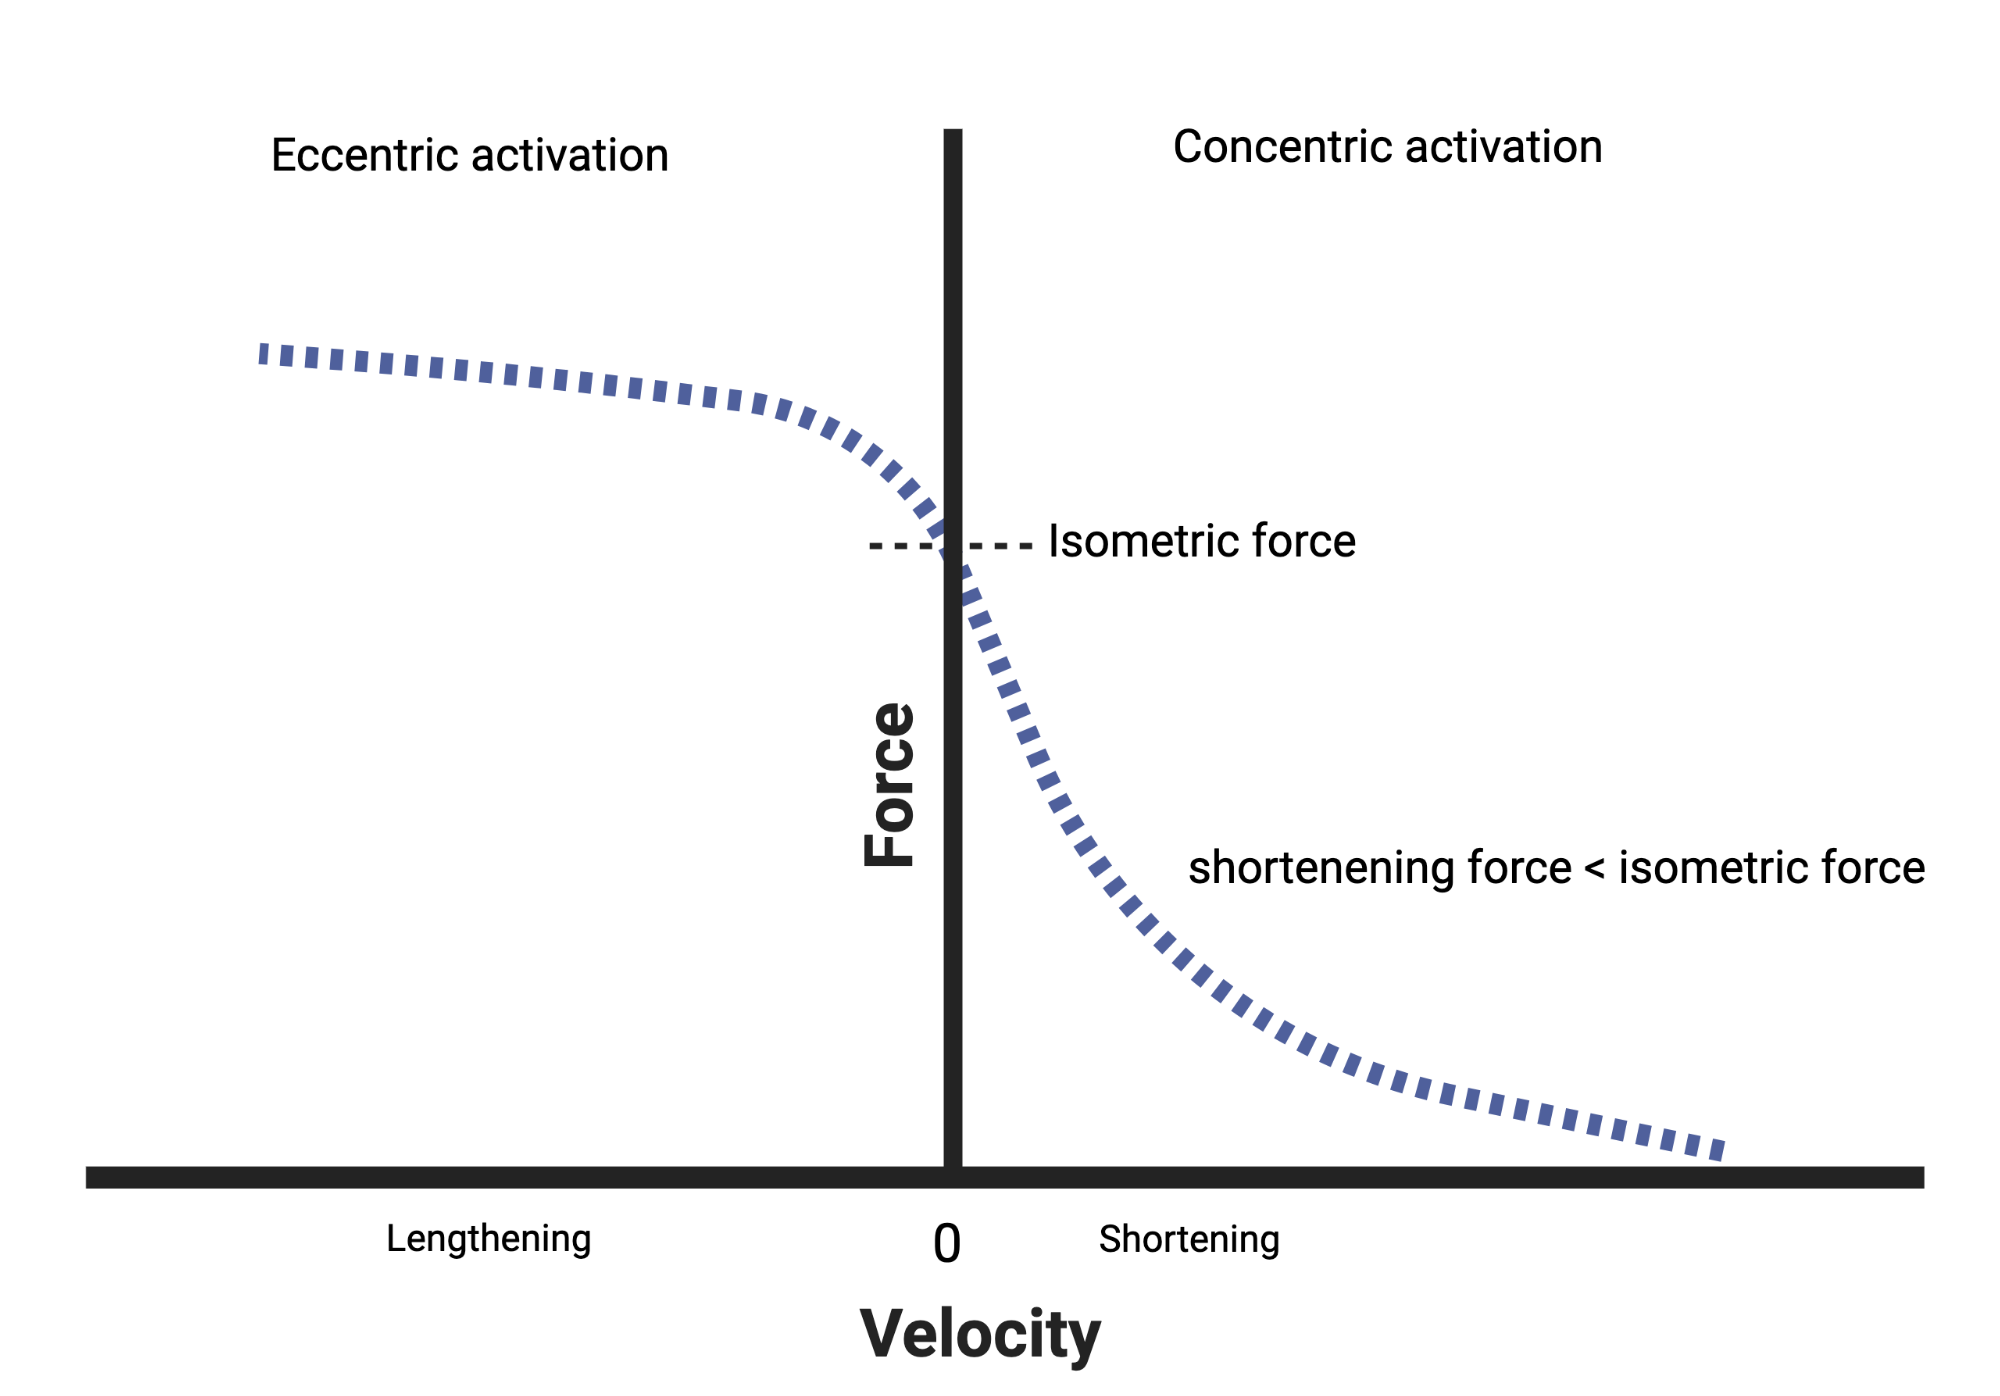
\includegraphics[width=1\linewidth]{./figure/force_velocity_lengthening.png}
    \caption{Force Velocity Curve during Shortening \footnotesize{(Created with Biorender.com}}
    \label{fig:force_velocity_lengthening}
\end{figure}


\paragraph{Experience of the FV relationship during eccentric activation}

The FV relationship during eccentric activation is something people can easily relate to and have experienced. Very simply, as the load someone attempts to hold  (but cannot actually hold) increases, the velocity of movement (muscles get longer) also increases.

\section{Summary \& Next Step}

In this chapter we have covered the micro anatomy of muscle fibers at sufficient depth to understand the mechanisms behind several concepts relevant for physical therapy practice such as the length tension and force velocity relationships. The sarcomere is the functional unit of the muscle cell due to its repeated appearance in the muscle.  You should now understand the parts and capabilities of muscle fibers at the level of the sarcomere and how these can generate active tension by converting chemical energy into mechanical energy, or passive tension by resisting change to length. Active tension involves a sequence of events repeated over and over. The sequence begins with excitation of the muscle fiber. Therefore, our next step is to consider excitation.

\printbibliography[heading=subbibintoc]
